\section{Kompleksitas}
\begin{figure}[H]
        \centerline{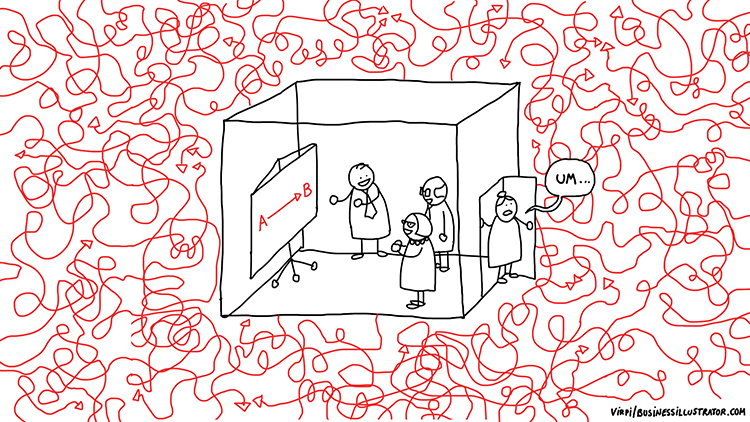
\includegraphics[scale=0.35]{figures/algoritma-kompleksitas/kompleksitas}}
        \caption{Kompleksitas}
\end{figure}
Kompleksitas adalah suatu indikator antarhubungan di dalam suatu program yang memengaruhi cara bagaimana hubungan ini akan dikelola dan keahlian yang dibutuhkan untuk mengelolanya. Semua program dihasilkan dari banyak fungsi dan proses yang saling berhubungan dimana semuanya sangat kompleks. Kompleksitas dibagi menjadi 2 yaitu Time Complexity dan Space Complexity.

\section{Asymptonic Noation}


\section{Big O Notation}
\begin{figure}[H]
        \centerline{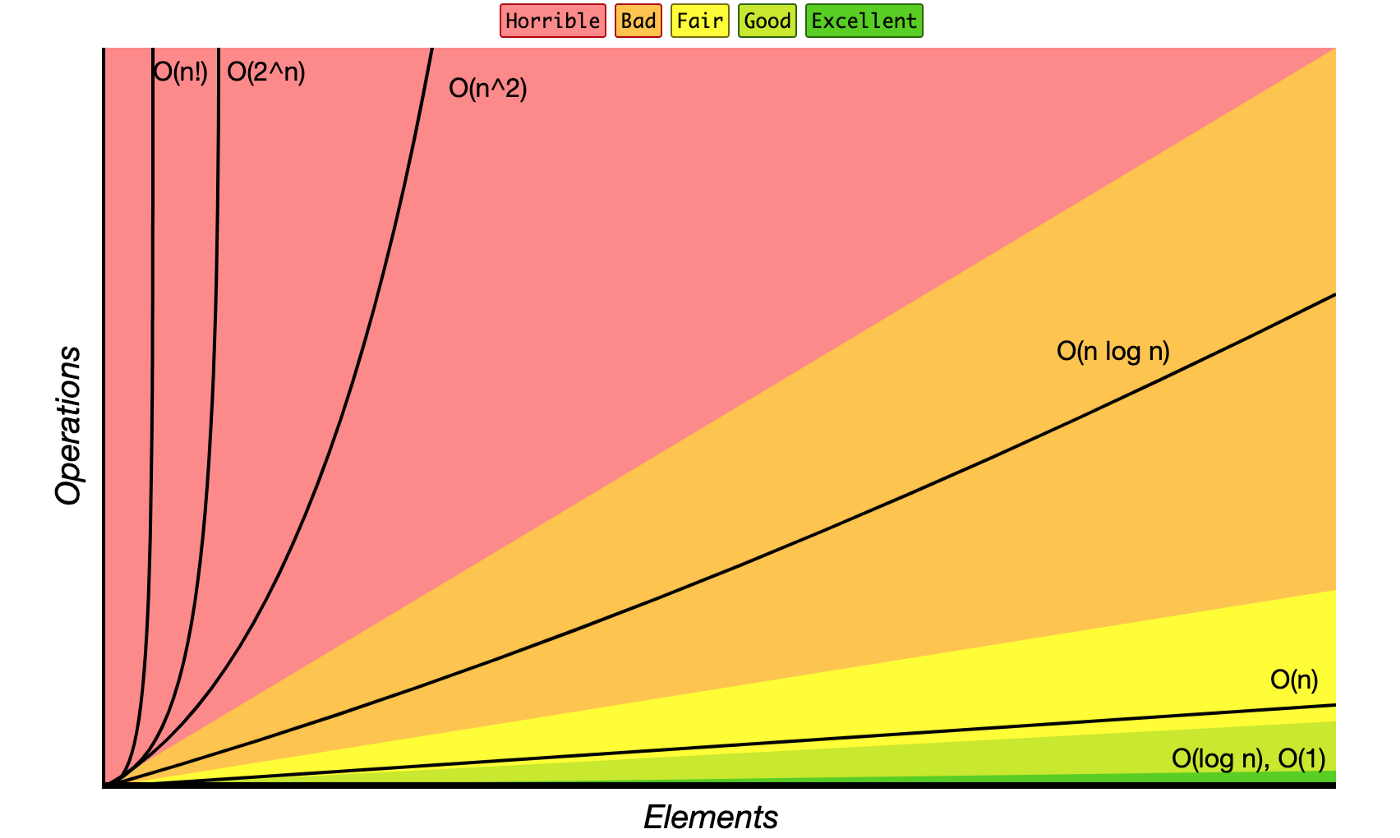
\includegraphics[scale=0.3]{figures/algoritma-kompleksitas/bigonotation}}
        \caption{Big O Notation}
\end{figure}
Big o notation dapat kita fahami sebagai notasi atau lambang matematika yang menggambarkan tingkat dari kompleksitas atau kerumitan suatu sistem. Big o notation biasanya dilambangkan sebagai O(n). Prinsip-prinsip big o notation ini dapat kita terapkan pada ilmu komputer untuk mengelompokkan atau mengklasifikasikan algoritma pemograman berdasarkan kerumitannya. Pada penerapannya, big o notasi ini mengukur tingkat lamanya waktu proses (running time) dan space atau resource yang digunakan berbading lurus dengan bertambahnya input data.

Big o notasi menjelaskan suatu fungsi yang diindentifikasi berdasarkan pertumbuhan datanya. Fungsi atau algoritma yang berbeda tetapi tingkat pertumbuhannya sama dapat dilambangkan dengan big o notasi yang sama. Para developer atau programmmer biasaanya mendifinisikan tingkat kerumitan code atau algoritma yang kita buat mengunakan big o notasi ini. Dengan demikian, hal ini memudahkan cara berkomunikasi yang baik antar programmer dalam membahas kerumitan suatu algoritma. Berikut adalah cheat sheet dari bebarapa operasi umum pada struktur data dalam bahasa pemograman.
\begin{figure}[H]
        \centerline{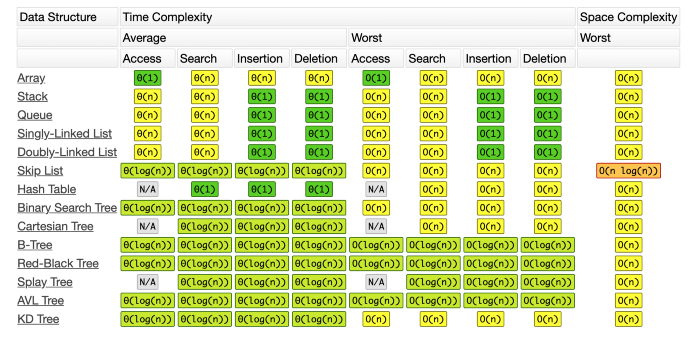
\includegraphics[scale=0.5]{figures/algoritma-kompleksitas/cheatsheetbigonotation}}
        \caption{Cheat Sheet Big O Notation}
\end{figure}

Sebagai cotoh, konsep arrray memiliki notasi O(1) untuk cara mengkases data dan O(n) untuk proses input data. Dari kedua grafik tersebut kita mendapatkan informasi bahwa konsep array ini memiliki performance terbaik untuk cara akses dan tidak terpengaruh terhadap banyaknya data. Adapun untuk proses insert data dia akan meningkat secara aritmetik dan prosesnya masih di bilang sangat bagus. Berikut data cheat sheet untuk teknik melakukan sorting dan nilai big o notasinya.
\begin{figure}[H]
        \centerline{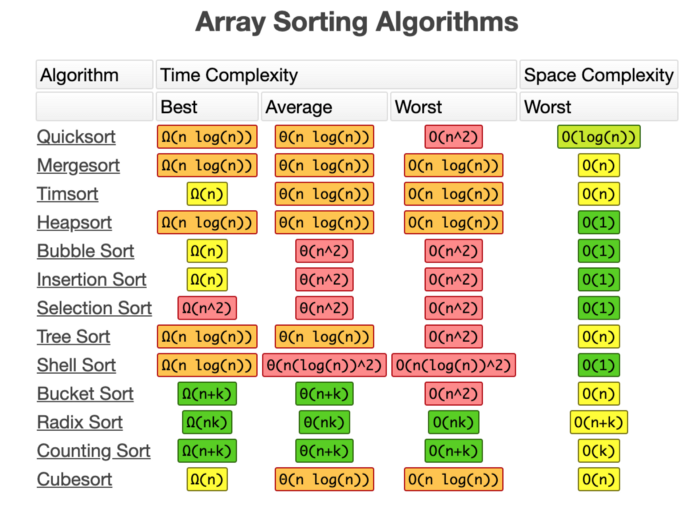
\includegraphics[scale=0.5]{figures/algoritma-kompleksitas/cheatsheetbigonotationsorting}}
        \caption{Cheat Sheet Big O Notation Sorting}
\end{figure}

\subsection{Cara Membaca dan Memahami Big O}
Kompleksitas dalam waktu artinya adalah seberapa lama kode program yang kita untuk menyelesaikan sebuah masalah yang kompleks. Kompleksitas ruang sama halnya dengan kompleksitas waktu, semakin rumit masalah yang ingin diselesaikan maka ruang sebagai penyimpanan atau bisa disebut memory akan semakin banyak digunakan. Dibawah ini ada contoh untuk membaca dan memahami Big O Notation dan penjelasannya.
\begin{enumerate}
\item O(log n) berarti tingkat kompleksitas akan berbanding lurus dengan log dari banyaknya jumlah data. Algoritma yang masuk kategori O(log n) maka algoritma tersebut masuk kekategori yang sangat bagus.
\item O(1) tingkat kompleksitas yang konstan dengan model grafik horizontal. Algoritma yang memiliki kategori O(1) adalah algoritma yang terbaik dikarenakan time complexity dan space complexity yang paling cepat dan sedikit memakan ruang memory.
\item O(n) tingkat kompleksitas yang linear atau berbanding lurus dengan banyaknya data sehingga akan membentuk garis diagonal. Dalam matematika bisa disebut linear.
\item O(n+2) atau O(2n+5) sama dengan tingkat kompleksitas O(n). Jadi konstanta tidak dimasukan dalam penghitungan tingkat kompleksitas.
\end{enumerate}

\subsection{Kegunaan Pemahaman Big O}
Akan muncul beberapa pertanyaan apakah teori Big O Notation akan berguna dalam kehidupan sehari-hari programmer atau hanya berguna ketika akan mengikuti test penerimaan kerja? Jawabannya adalah ya untuk kedua kondisi tersebut. Pada penggunaan sehari-hari pengetahaun big o notasi ini akan sangat berguna dalam meningkatkan kualitas serta performance dari algoritma-algoritma yang kita buat. Kita sebagai programmer atau penulis kode program akan mengetahui seberapa cepat atau bisa dibilang Time Complexity dari kode program yang kita tulis ketika data yang diproses semakin besar.

\subsection{Contoh Big O Notasi dengan Python3}

\subsubsection{O(1)}
O(1) adalah Big O Notasi paling baik diantara semua kategori dikarenakan O(1) konstan sehingga tidak memiliki tambahan operasi apapun untuk menambah waktu apapun. O(1) terdiri dari operasi sedarhana yang tidak membutuhkan iterasi atau perulangan dalam kode program, contohnya adalah sebagai berikut.
\begin{lstlisting}[language=Python]
ini_list = ['tri', 'angga', 'dio', 'simamora']
_ = ini_list[0]
\end{lstlisting}
Kode program Python diatas akan masuk ke kategori O(1) dikarenakan kode program mengetahui index yang akan dituju dalam hal ini index 0 yang berisi 'tri'.

\subsubsection{O(log n)}
O(log n) adalah kategori Big O Notatio yang berada dibawah O(1) dikarenakan ketegori Big O Notasi ini memiliki iterasi dan setiap iterasinya akan dilipat menjadi 2 (kurang, tambah, bagi, kali), berikut contohnya.
\begin{lstlisting}[language=Python]
t = 100
while t > 10:
    t -= 10
\end{lstlisting}
Input n sebesar 100 akan tetapi dalam iterasi dikurangi 10 sehingga perulangan bisa diakhiri dengan lebih cepat.

\subsubsection{O(n)}
O(n) adalah Big O Notasi yang sering kita terapkan dalam kode program, O(n) adalah kategori iterasi dalam kode program yang menggunakan seluruh element n yang diberikan, berikut contohnya
\begin{lstlisting}[language=Python]
ini_list = ['tri', 'angga', 'dio']
for i in ini_list:
    print(i)
\end{lstlisting}
Kode program diatas adalah salah satu contoh penggunaan O(n), banyak sekali library built in python yang mengadopsi O(n) contohnya adalah ketika kita ingin mengetahui sebuah index dari list berdasarkan nilainya maka kode program tersebut akan masuk kekategori O(n) mengapa demikian? mari kita coba
\begin{lstlisting}[language=Python]
# ada 1 built in pada python yaitu .index() untuk menemukan index ke berapa berdasarkan nilai, mari kita bedah mengapa bisa masuk kategori O(n)

ini_list = ['tri', 'angga', 'dio']

index_tri = ini_list.index('tri') # maka akan berisi 0

# berikut kode searchnya
def get_index(value_search):
    index = 0
    list_data = ['tri', 'angga', 'dio', 'simamora']
    for value in list_data:
        if value == value_search:
            return index
        index += 1
    return None
\end{lstlisting}
Bisa terlihat untuk list search dengan pengembalian dimana index itu berada masuk dalam kategori O(n)

\subsection{O($n^2$)}
O($n^2$) bisa dibilang kategori yang semestinya dihindarkan jika ingin mengolah data yang banyak, dikarenakan O($n^2$) memiliki perulangan didalam perulangan, atau bisa dibilan nested loops. Nested loop akan aman digunakan jika data yang digunakan sangat sedikit, akan tetapi jika data yang diolah mencapai jutaan maka kategori O($n^2$) harus dipertimbangkan dalam penggunaannya. Berikut contoh kode program O($n^2$).
\begin{lstlisting}[language=Python]
ini_list_list = [['tri', 0], ['angga', 1], ['dio', 2], ['simamora', 3]]
value = 'dio'
for i in ini_list_list:
    for j in i:
        if j == value:
            print(i[1])
            break
    else:
        continue
    break
\end{lstlisting}

\subsection{Ingin merasakan perbedaan dari O(n) dan O($n^2$) ????}
Jika anda penasaran apa yang saya maksud jika mengolah data yang besar, mari kita coba. Jika anda sudah memiliki akun Github, dan sudah mengikuti semua tutorial Github diatas maka anda sudah bisa mengikuti tutorial ini, jika belum maka anda harus menyelesaikan tutorial diatas. Markicob (mari kita coba)

\begin{enumerate}
\item kunjungi Github Repository \footnote[1]{\url{https://github.com/trianggadios/data-preprocessing-computational}}, maka akan muncul seperti dibawah ini.
\begin{figure}[H]
        \centerline{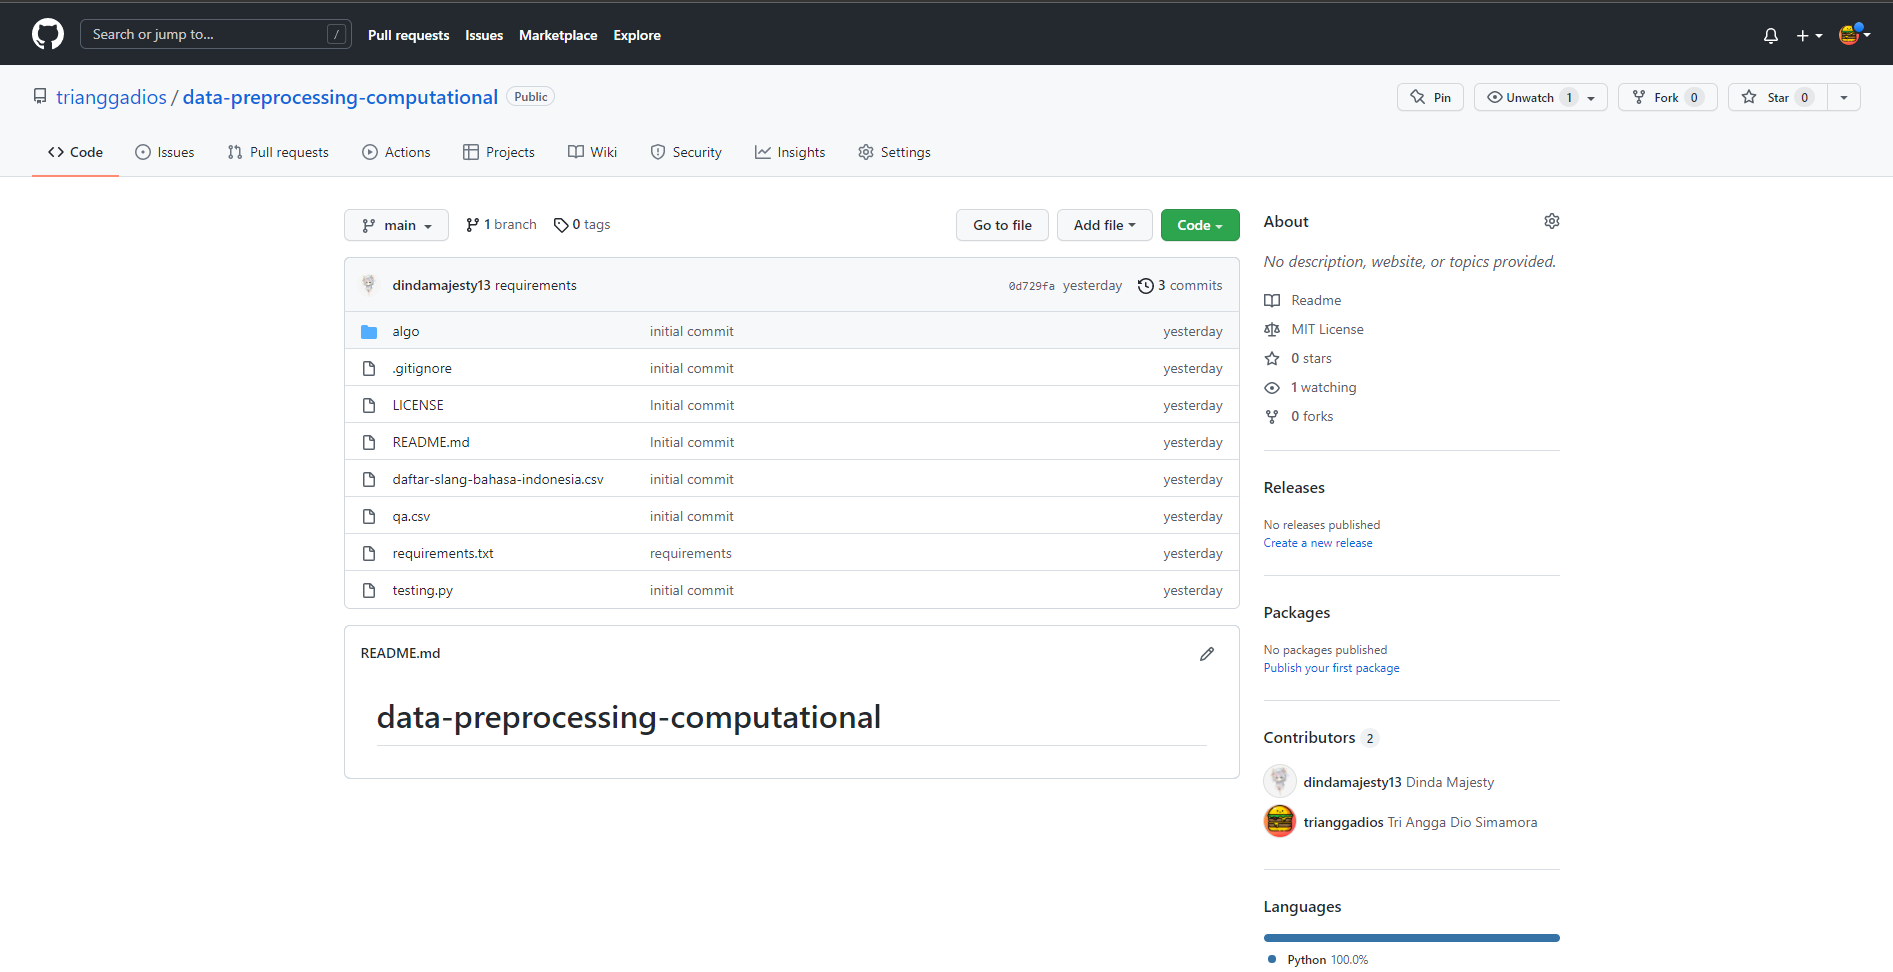
\includegraphics[scale=0.35]{figures/mencoba-computational/step1}}
        \caption{Mencoba Big O Notation: Step 1}
\end{figure}
\item setelah itu klik bagian Code dan klik logo copy hingga ada tulisan \textbf{Copied!}
\begin{figure}[H]
        \centerline{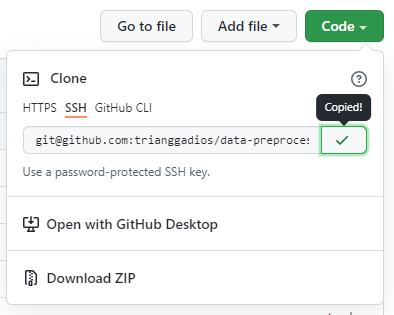
\includegraphics[scale=0.35]{figures/mencoba-computational/step2}}
        \caption{Mencoba Big O Notation: Step 2}
\end{figure}
\item buka git bash anda, lalu ketikkan \textbf{git clone [url yang sudah dicopy bisa dipaste]}, tekan enter
\begin{figure}[H]
        \centerline{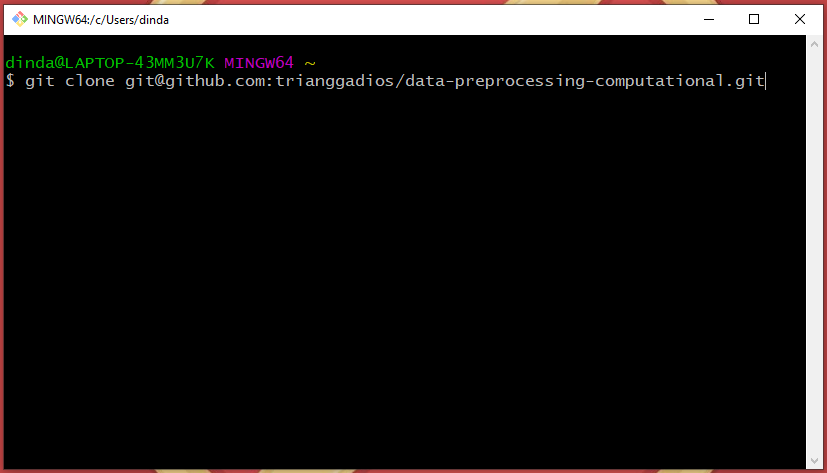
\includegraphics[scale=0.35]{figures/mencoba-computational/step3}}
        \caption{Mencoba Big O Notation: Step 3}
\end{figure}
\item tunggu hingga selesai
\begin{figure}[H]
        \centerline{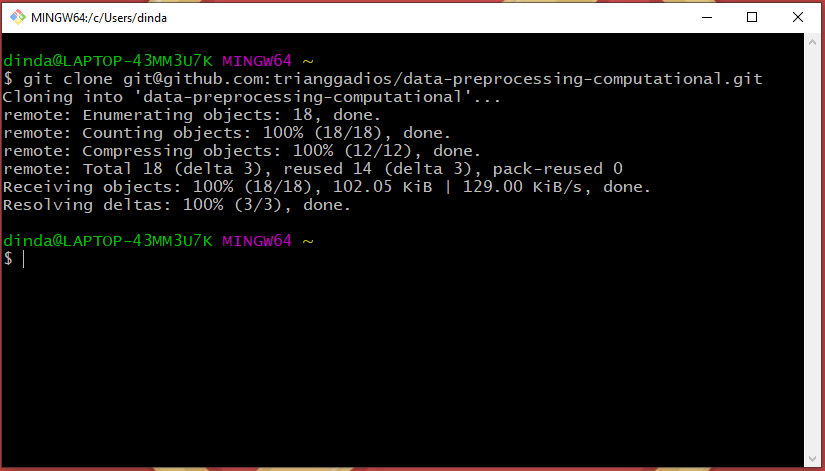
\includegraphics[scale=0.35]{figures/mencoba-computational/step4}}
        \caption{Mencoba Big O Notation: Step 4}
\end{figure}
\item lalu masuk ke directory dengan mengetikkan \textbf{cd data-preprocessing-computational/}, tekan enter
\begin{figure}[H]
        \centerline{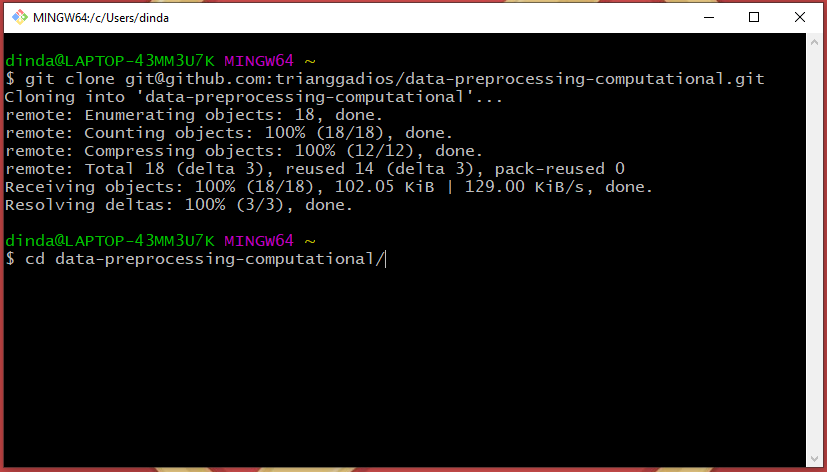
\includegraphics[scale=0.35]{figures/mencoba-computational/step5}}
        \caption{Mencoba Big O Notation: Step 5}
\end{figure}
\item lalu ketikkan perintah berikut ini \textbf{pip install -r requirements.txt}, tekan enter, tunggu hingga selesai
\begin{figure}[H]
        \centerline{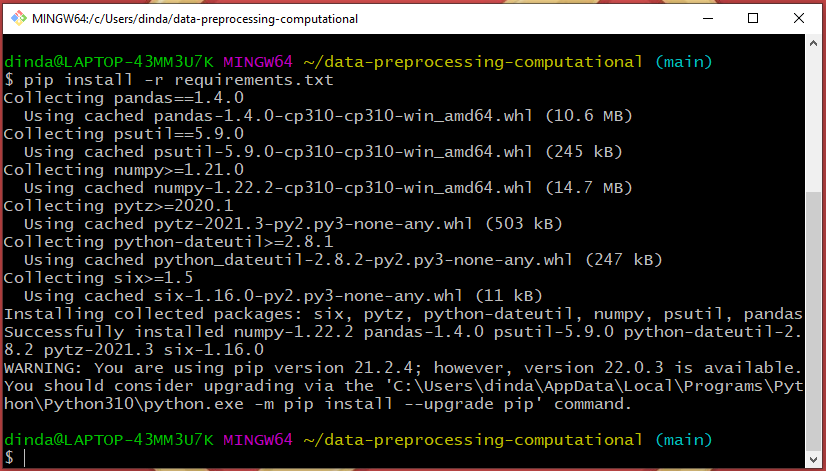
\includegraphics[scale=0.35]{figures/mencoba-computational/step6}}
        \caption{Mencoba Big O Notation: Step 6}
\end{figure}
\item lalu jalankan script python dengan mengetikkan \textbf{python testing.py}, tekan enter, tunggu hingga kode program selesai
\begin{figure}[H]
        \centerline{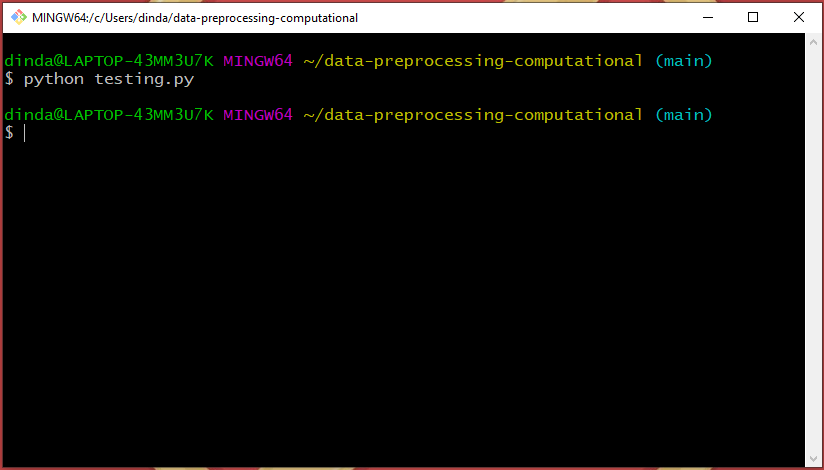
\includegraphics[scale=0.35]{figures/mencoba-computational/step7}}
        \caption{Mencoba Big O Notation: Step 7}
\end{figure}
\item terdapat 2 algo yaitu algo1 dan algo2, algo1 menggunakan O($n^2$) sedangkan algo2 menggunakan O(n)
\item untuk melihat hasil kompleksitas waktu bisa mengetikkan perintah berikut, \textbf{cat algo1\_time.txt}
\begin{figure}[H]
        \centerline{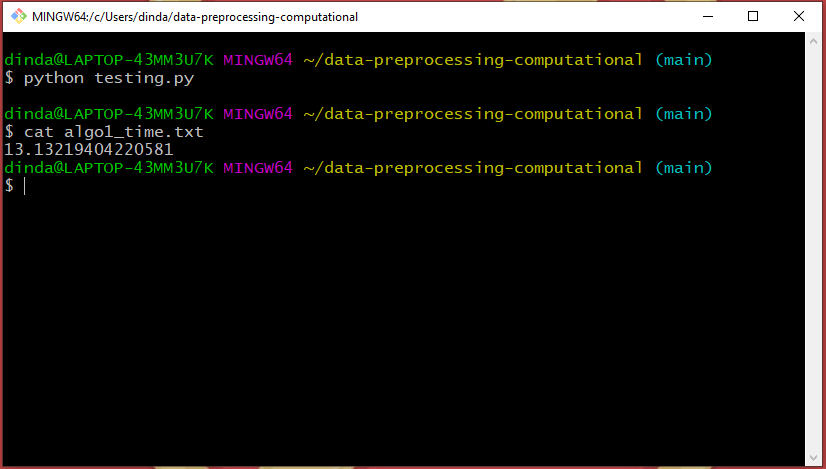
\includegraphics[scale=0.35]{figures/mencoba-computational/step8}}
        \caption{Mencoba Big O Notation: Step 8}
\end{figure}
\item terlihat gambar diatas yaitu hasil komputasi O($n^2$) yaitu 13 detik
\item jika ingin mengetahui berapa detik yang dihasilkan oleh O(n), ketikkan perintah berikut \textbf{cat algo2\_time.txt}, tekan enter
\begin{figure}[H]
        \centerline{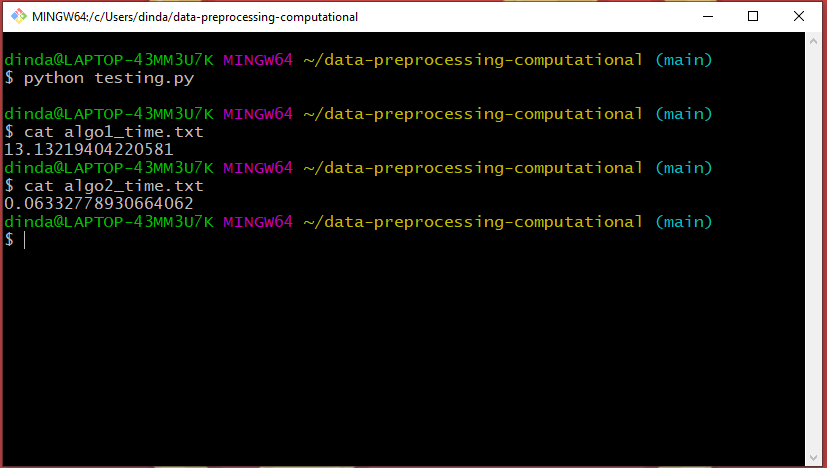
\includegraphics[scale=0.35]{figures/mencoba-computational/step9}}
        \caption{Mencoba Big O Notation: Step 9}
\end{figure}
\item sangat berbeda jauh bukan? mungkin akan tidak terasa jika data yang diolah sangat kecil akan tetapi jika menggunakan data yang besar maka akan terlihat sangat jauh perbedaannya.
\end{enumerate}